\section{NSW Readout Electronics and Detector Instrumentation}
\label{sec:nsw_elx}

To a very large extent, high-performance detectors are realised and made
possible only by their interfacing to equally high-performance readout electronics;
that is, high quality electronics enable high quality detectors.
In this section, therefore, an introduction to the frontend electronics\footnote{`Frontend' electronics
are those housed directly on the detectors themselves and are responsible for reading out the
detector signals and potentially many other responsibilities, such as calibration, configuration, and
detector controls (temperature monitoring, etc...). `Backend' electronics refer to those
not necessarily located in the experimental cavern housing the detectors but are in the nearby
service areas or on the surface (c.f. Figure~\ref{fig:p1}) and are dedicated, for example, to the implementation of detector trigger logic
and data decoding and event building (i.e. gathering all data from detector hits associated with a given event).}
relevant to the NSW will be given.
There is a large set of both frontend and backend electronics specifically
designed and constructed for the NSW~\cite{NSWFrontEndChristos}.
Here, though, we will focus primarily on the frontend electronics.
The NSW frontend electronics revolve around the operation of a family
of rather complex application specific integrated circuits (ASICs),
each targetting a specific (set of) purpose(s) related to data-acquisition or
constructing trigger primitives:

\begin{description}
    \item[] \textbf{VMM}~\cite{VMM1GDG,VMMASIC,VMM3George} Frontend readout ASIC used for precision and fast trigger data signal collection in both MM and sTGC detectors\footnote{The acronym for which `VMM' stands is not informative as in the case of the other NSW ASICs.
The `V' in VMM refers to the first initial of Venetios Polychronakos who is an ATLAS physicist involved
in the VMM design, among many other things. The `MM' in VMM refers to the MM detectors.
The reason for this acronym is the tradition of the main designer of the VMM, Gianluigi De Geronimo,
to name his projects based on the initial person requesting the project to be designed and that project's
purpose.
}
    \item[] \textbf{ROC}~\cite{NSWTDR,NSWFrontEndChristos} `ReadOut Controller' ASIC, responsible for buffering and aggregating precision data from the VMM
    \item[] \textbf{TDS}~\cite{TDS} `Trigger Data Serializer' ASIC, processes trigger signals from VMMs on the sTGC detectors and prepares trigger primitives for the NSW Level-1 muon trigger logic
    \item[] \textbf{ART}~\cite{NSWTDR,ARTASIC} 'Address in Real Time' ASIC, processes trigger signals from VMMs on the MM detectors and prepares trigger primitives for the NSW Level-1 muon trigger logic
\end{description}

The VMM ASIC is the primary ASIC of the NSW: all other ASICs listed above take as input
the outputs of the VMM and, in this respect, are secondary.
The work of the current author on the NSW frontend electronics is based almost exclusively
on the characterisation and validation of the VMM ASIC.
For these reasons, focus will be given on describing the VMM in Section~\ref{sec:vmm}.
For the interested reader, further information on the ROC, TDS, and ART ASICs is
provided in the references above.
The interface of the NSW frontend electronics to the associated detectors is dictated for the most part
by the geometry, type, and number of the detectors' readout elements (MM: strips, sTGC: strips, wires, and pads)
and foreseen space limitations in the ATLAS detector.
The work in the present thesis concerns the frontend boards related to the MM detectors.
This is mainly due to the fact that the VMM was initially conceptualised as a frontend ASIC specialised
for MPGD detectors and its initial prototypes were studied under this context by the RD51 collaboration
at CERN which is devoted to the development of MPGD technologies, such as the MM detectors.\footnote{For more information
on the RD51 collaboration, visit their homepage: \url{http://rd51-public.web.cern.ch/rd51-public/}.}
In Section~\ref{sec:nsw_boards}, then, a description of the relevant front-end boards used in the
study, validation, and integration of the VMM ASIC, as well as those that will be used in
the MM detectors of the NSW, will be given.
The analogous VMM-based frontend boards for the sTGC detectors are objectively more complicated than those
of the MM detectors for purely technical and uninteresting reasons.
The discussion below, however, is detector-technology agnostic and
the sTGC frontend description can be found elsewhere~\cite{NSWTDR}.

\subsection{The VMM ASIC}
\label{sec:vmm}

The VMM is a custom ASIC that can be used in a variety of charge-interpolated tracking
detectors.
There have been several iterations of the VMM over the years, starting with the VMM1~\cite{VMM1GDG} and
moving up to the VMM3~\cite{VMMASIC,VMM3George}.
An illustration of the evolution of complexity of the VMM ASIC is shown in Figure~\ref{fig:vmms_silicon}.
The VMM1 was a purely analog readout ASIC considered to be a prototype of the initial VMM functionalities.
The VMM2 was an extensive upgrade of the VMM1, adding the necessary digital logic and functional blocks
required for the NSW detectors.
The VMM3 is the final version of the ASIC\footnote{In actuality, there have been two versions of the
VMM3: the VMM3 and the `VMM3a'. The VMM3a is the true final version that will be used in the NSW
and addresses issues found during the testing and validation of the first round of the VMM3 production}
providing enhanced functionality required for data taking in ATLAS
as well as addressing bugs found in the operation of the VMM2.
VMM3 is the version that will be used
in the NSW once installed in ATLAS.
The VMM implements all logic using triple modular redundancy (TMR) to protect itself
from single event upsets (SEUs) that are expected to be quite common in the
harsh radiation environments in which the NSW will be situated.

The VMM is composed of 64 discrete frontend channels, each to be connected to a detector
readout element.
A block diagram illustrating the functional blocks of the VMM3 and its channels is
shown in Figure~\ref{fig:vmm3_channel}.
Each channel has a dedicated charge amplifier (`CA' in Figure~\ref{fig:vmm3_channel}) and signal
shaping functionality,
threshold discriminator, test-pulse injection capacitor with adjustable amplitude provided
by a 10-bit digital-to-analog converter (DAC), and precise signal amplitude and timing measurements digitally readout via
internal per-channel analog-to-digital converters (ADCs).
The amplitude measurement of the input pulse is digitised by a 10-bit ADC (`PDO', for `peak detector output', in Figure~\ref{fig:vmm3_channel})
and the timing estimation of the signal pulse's peak is digitised by an 8-bit ADC (`TDO', for `time detector output', in Figure~\ref{fig:vmm3_channel}).
The digitised output of these amplitude and timing measurements are calculated by these
internal ADCs within 200\,ns and stored in internal buffers of the VMM.
The buffered data is stored until selected for readout by another ASIC housed on the same frontend
board as the VMM, the ROC, based on the buffered data's associated bunch crossing.
The PDO and TDO data are those used in the precision hit reconstruction in the detectors.
The hit timing information provided by the TDO is critical only for the MM detectors which
rely primarily on the $\mu$-TPC hit reconstruction method, as illustrated in Figure~\ref{fig:mm_tpc_hit_loc}.
For the sTGC, the accurate timing information is not required for precision tracking and,
to increase readout bandwidth, the timing information will likely not be serialised
in the data output from the sTGC frontend electronics.

In addition to the precision data useful for reconstructing high-level muon tracks provided by
the PDO and TDO measurements, the VMM can also operate at a faster mode used for
providing data needed for the building of trigger primitives.
In the trigger mode referred to as the `Address-in-Real-Time' (ART) mode,
the VMM outputs the \textit{first} channel address (e.g. MM strip number) on which
an above-threshold peak was detected.
An alternative trigger mode relies on the VMM's ability to perform a fast digitisation of
the signal pulse amplitude using a 6-bit ADC, providing a coarse but rapid measurement
of the signal amplitude.
Additionally, the VMM can output fast timing signals, such as a flag indicating a signal over threshold (`Time-Over-Threshold', or TOT as in Figure~\ref{fig:vmm3_channel}).
The ART trigger scheme is used for the MM trigger primitives and the combination
of the coarse 6-bit amplitude and fast-timing signals is used for building the
sTGC trigger primitives.

One of the powers of the VMM is its highly configurable nature.
This, of course, makes the ASIC quite complex in terms of its design but is
advantageous in terms of its range usefulness.
Some of the main configurable items are the peaking (integration) time of the signal shaper
(25, 50, 100, and 200\,ns), adjustable thresholds per-VMM configured by an on-VMM
10-bit (DAC),
adjustable channel gains (0.5, 1, 3, 4.5, 6, 9, 12, and 16\,mV/fC),
time-to-amplitude conversion (TAC) ramp time (60, 100, 350, and 650\,ns) relevant for the timing measurements,
and channel threshold trimmers provided by 5-bit DACs that adjust each channel's individual
threshold around the globally-configured (per-VMM) threshold.
The VMM input can also be configured to handle either positive or negative input
signals.
This latter fact is necessary for the NSW, in which the sTGC and MM detectors
will induce signals of opposite polarity on their readout elements.\footnote{The MM strips and
sTGC wires produce signals of opposite polarity as the sTGC strips and pads.}

\begin{figure}[!htb]
    \begin{center}
        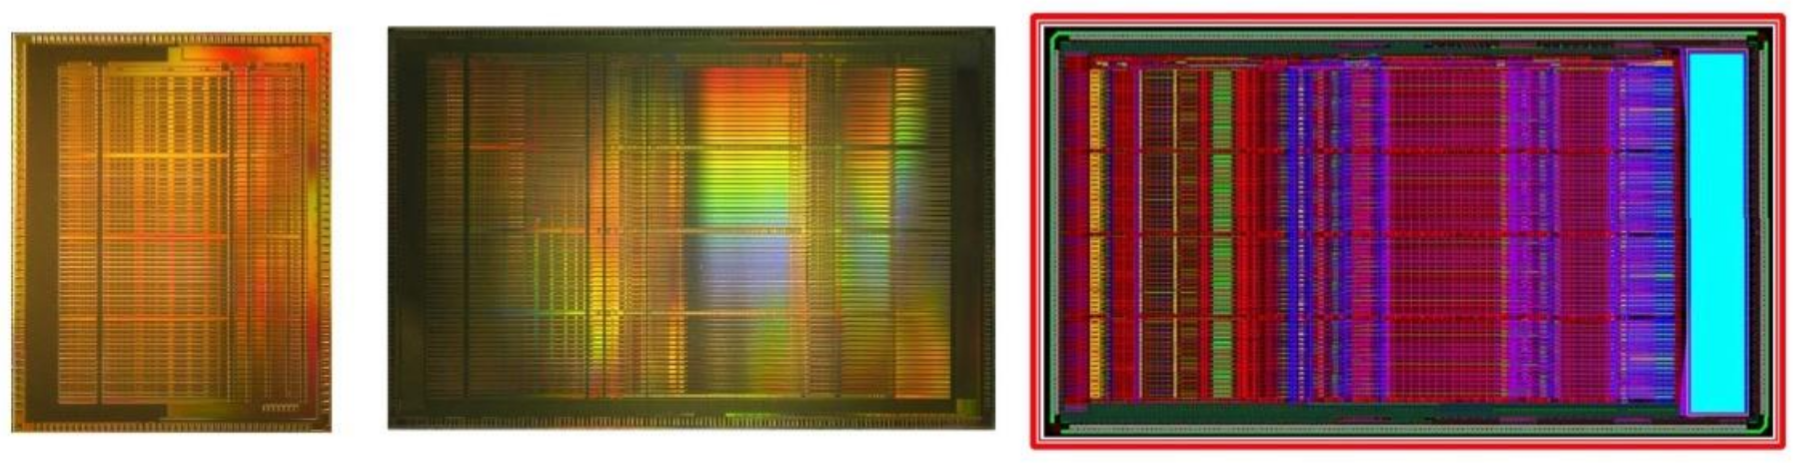
\includegraphics[width=0.8\textwidth]{figures/nsw/vmm/vmms_silicon}
        \caption{
            Evolution of the VMM ASIC.
            Shown are the silicon dies or routing of the the VMM1 (\textbf{\textit{left}}), to the VMM2 (\textbf{\textit{middle}}), and 
            the VMM3 (\textbf{\textit{right}}), the final version that will be used in the NSW.
            The VMM1 has an area of 50\,mm$^2$ with $\approx 500$\,k MOSFETs, the VMM2 area is 115\,mm$^2$ with $>5$\,M MOSFETs,
            and the VMM3 area is 130\,mm$^2$ with $>6$\,M MOSFETs.\protect\footnotemark%
        }
        \label{fig:vmms_silicon}
    \end{center}
\end{figure}
\footnotetext{`MOSFET' stands for metal-oxide-semiconductor field-effect  transistor', the most widely used transistor in digital and analog electronics.}

\begin{figure}[!htb]
    \begin{center}
        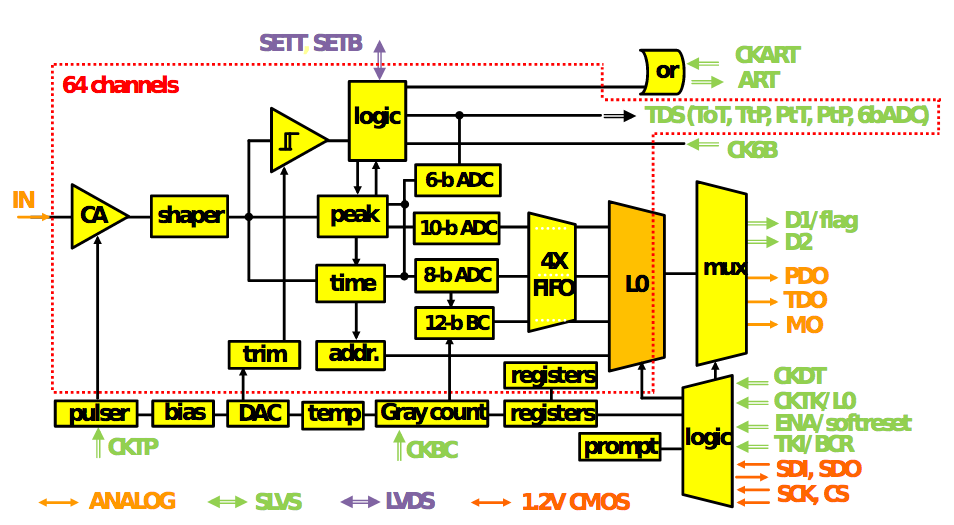
\includegraphics[width=0.8\textwidth]{figures/nsw/vmm/vmm3_channel}
        \caption{
            Architecture of the VMM3.
            The items contained within the dotted red line are repeated
            for each of the 64 channels of the VMM.
            Figure taken from Ref.~\cite{VMM3George}.
        }
        \label{fig:vmm3_channel}
    \end{center}
\end{figure}

\subsection{Frontend-electronics Boards for the NSW}
\label{sec:nsw_boards}

There have been two classes of frontend boards encountered
throughout the work on the NSW electronics represented in this thesis.
The first class relates to a type of frontend board that is not specific to the NSW
but which houses one (or several) VMM ASICs.
The second class relates to prototype frontend boards following the design to be used
in the NSW to readout the MM detectors, the so-called MMFE8 frontend board.
Figure~\ref{fig:frontend_boards} provides pictures of these two classes of frontend
boards with relevant parts indicated.

The general purpose frontend boards, such as the GPVMM in Figure~\ref{fig:frontend_boards}, are those used primarily for the direct study
and characterisation of the VMM ASIC.
The prototype MMFE8 frontend boards allow for a more realistic interface to the MM
detectors to be studied as well as for the overall design and layout of the hardware components on the
boards themselves to be studied and optimised.
One such optimisation was the placement of the DC-to-DC converters used for the on-board power distribution.\footnote{In the
final MMFE8 prototype frontend boards, and in those to be used in the NSW,
the DC-to-DC converters are packaged in the so-called FEAST ASIC developed by CERN.
Further information at \url{https://project-dcdc.web.cern.ch/project-dcdc/Default.html}}
DC-to-DC converters are potential sources of electronic noise and stray electromagnetic fields as a result of
their high switching frequencies.
When placed directly on the frontend boards, their proximity to the sensitive readout
elements means that the matter of their placement and shielding needs to be handled carefully.

The types of boards discussed here have allowed for the study of the VMM ASIC both on- and off-detector,
where in the latter case prototype MM detectors were used.
Over the timespan of the present thesis, many iterations of each type of frontend board
were encountered, with subsequent iterations adapting to the evolution of the VMM, for example (Figure~\ref{fig:vmms_silicon}).
In addition to housing the VMM ASIC, the frontend boards house a
\textsc{Xilinx} field-programmable gate array (FPGA). 
One of the main purposes of the FPGA is to aggregate the data being output from the VMM
and prepare it for being sent off board via standard network protocols over Ethernet to the
backend data-acquisition system. 
Additionally, the FPGA responds to commands and requests submitted by users via the software
interface.
Such commands may have as endpoint the FPGA itself or they may require the FPGA to forward
them to the VMM ASIC.
These concepts are described further in Section~\ref{sec:verso}.

The GPVMM board has a simple connector designed in such a way that lends itself to
be easily adapted to many types of detectors in labs and teststands.
The MMFE8 board, both the prototypes and those to be used in the NSW, use a ZEBRA\footnote{More information
on ZEBRA-type connectors can be found online at \url{https://en.wikipedia.org/wiki/Elastomeric_connector}} elastomeric
connector that allows for a seamless interconnect between the readout strips on the MM detector layers
and the VMM channel inputs.
The principle of the ZEBRA connector is illustrated in Figure~\ref{fig:zebra_connector}.

\begin{figure}[!htb]
    \begin{center}
        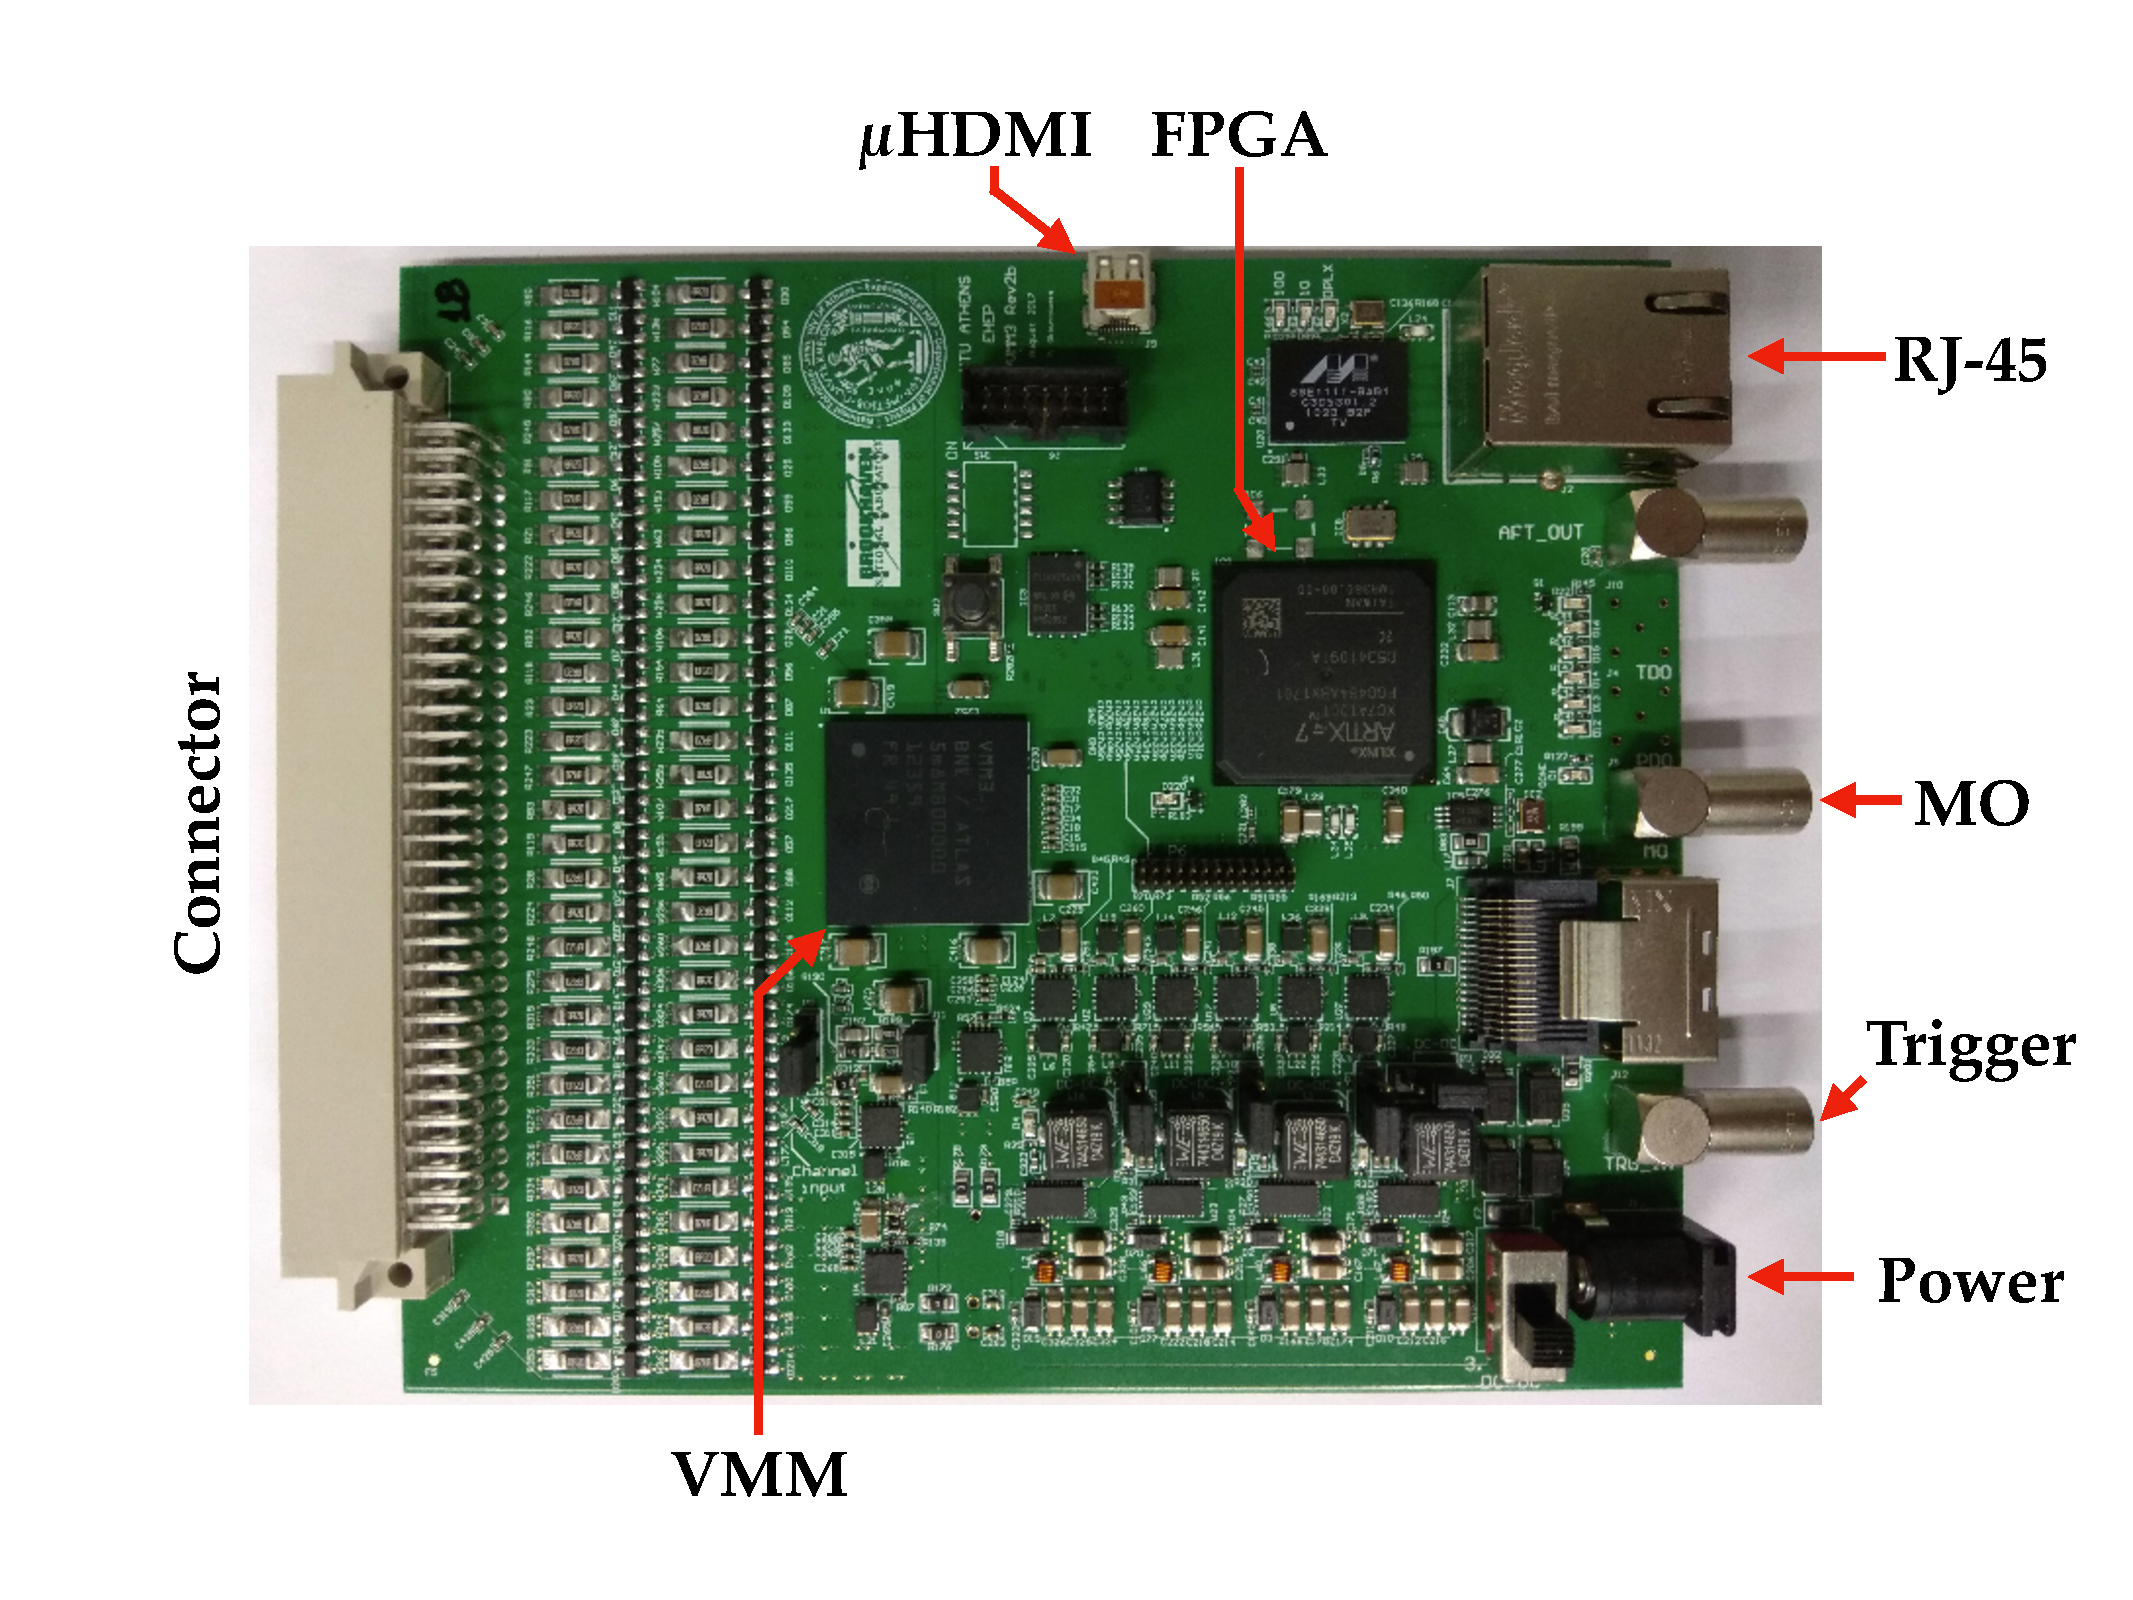
\includegraphics[width=0.8\textwidth]{figures/nsw/frontend/gpvmm_labelledPDF}
        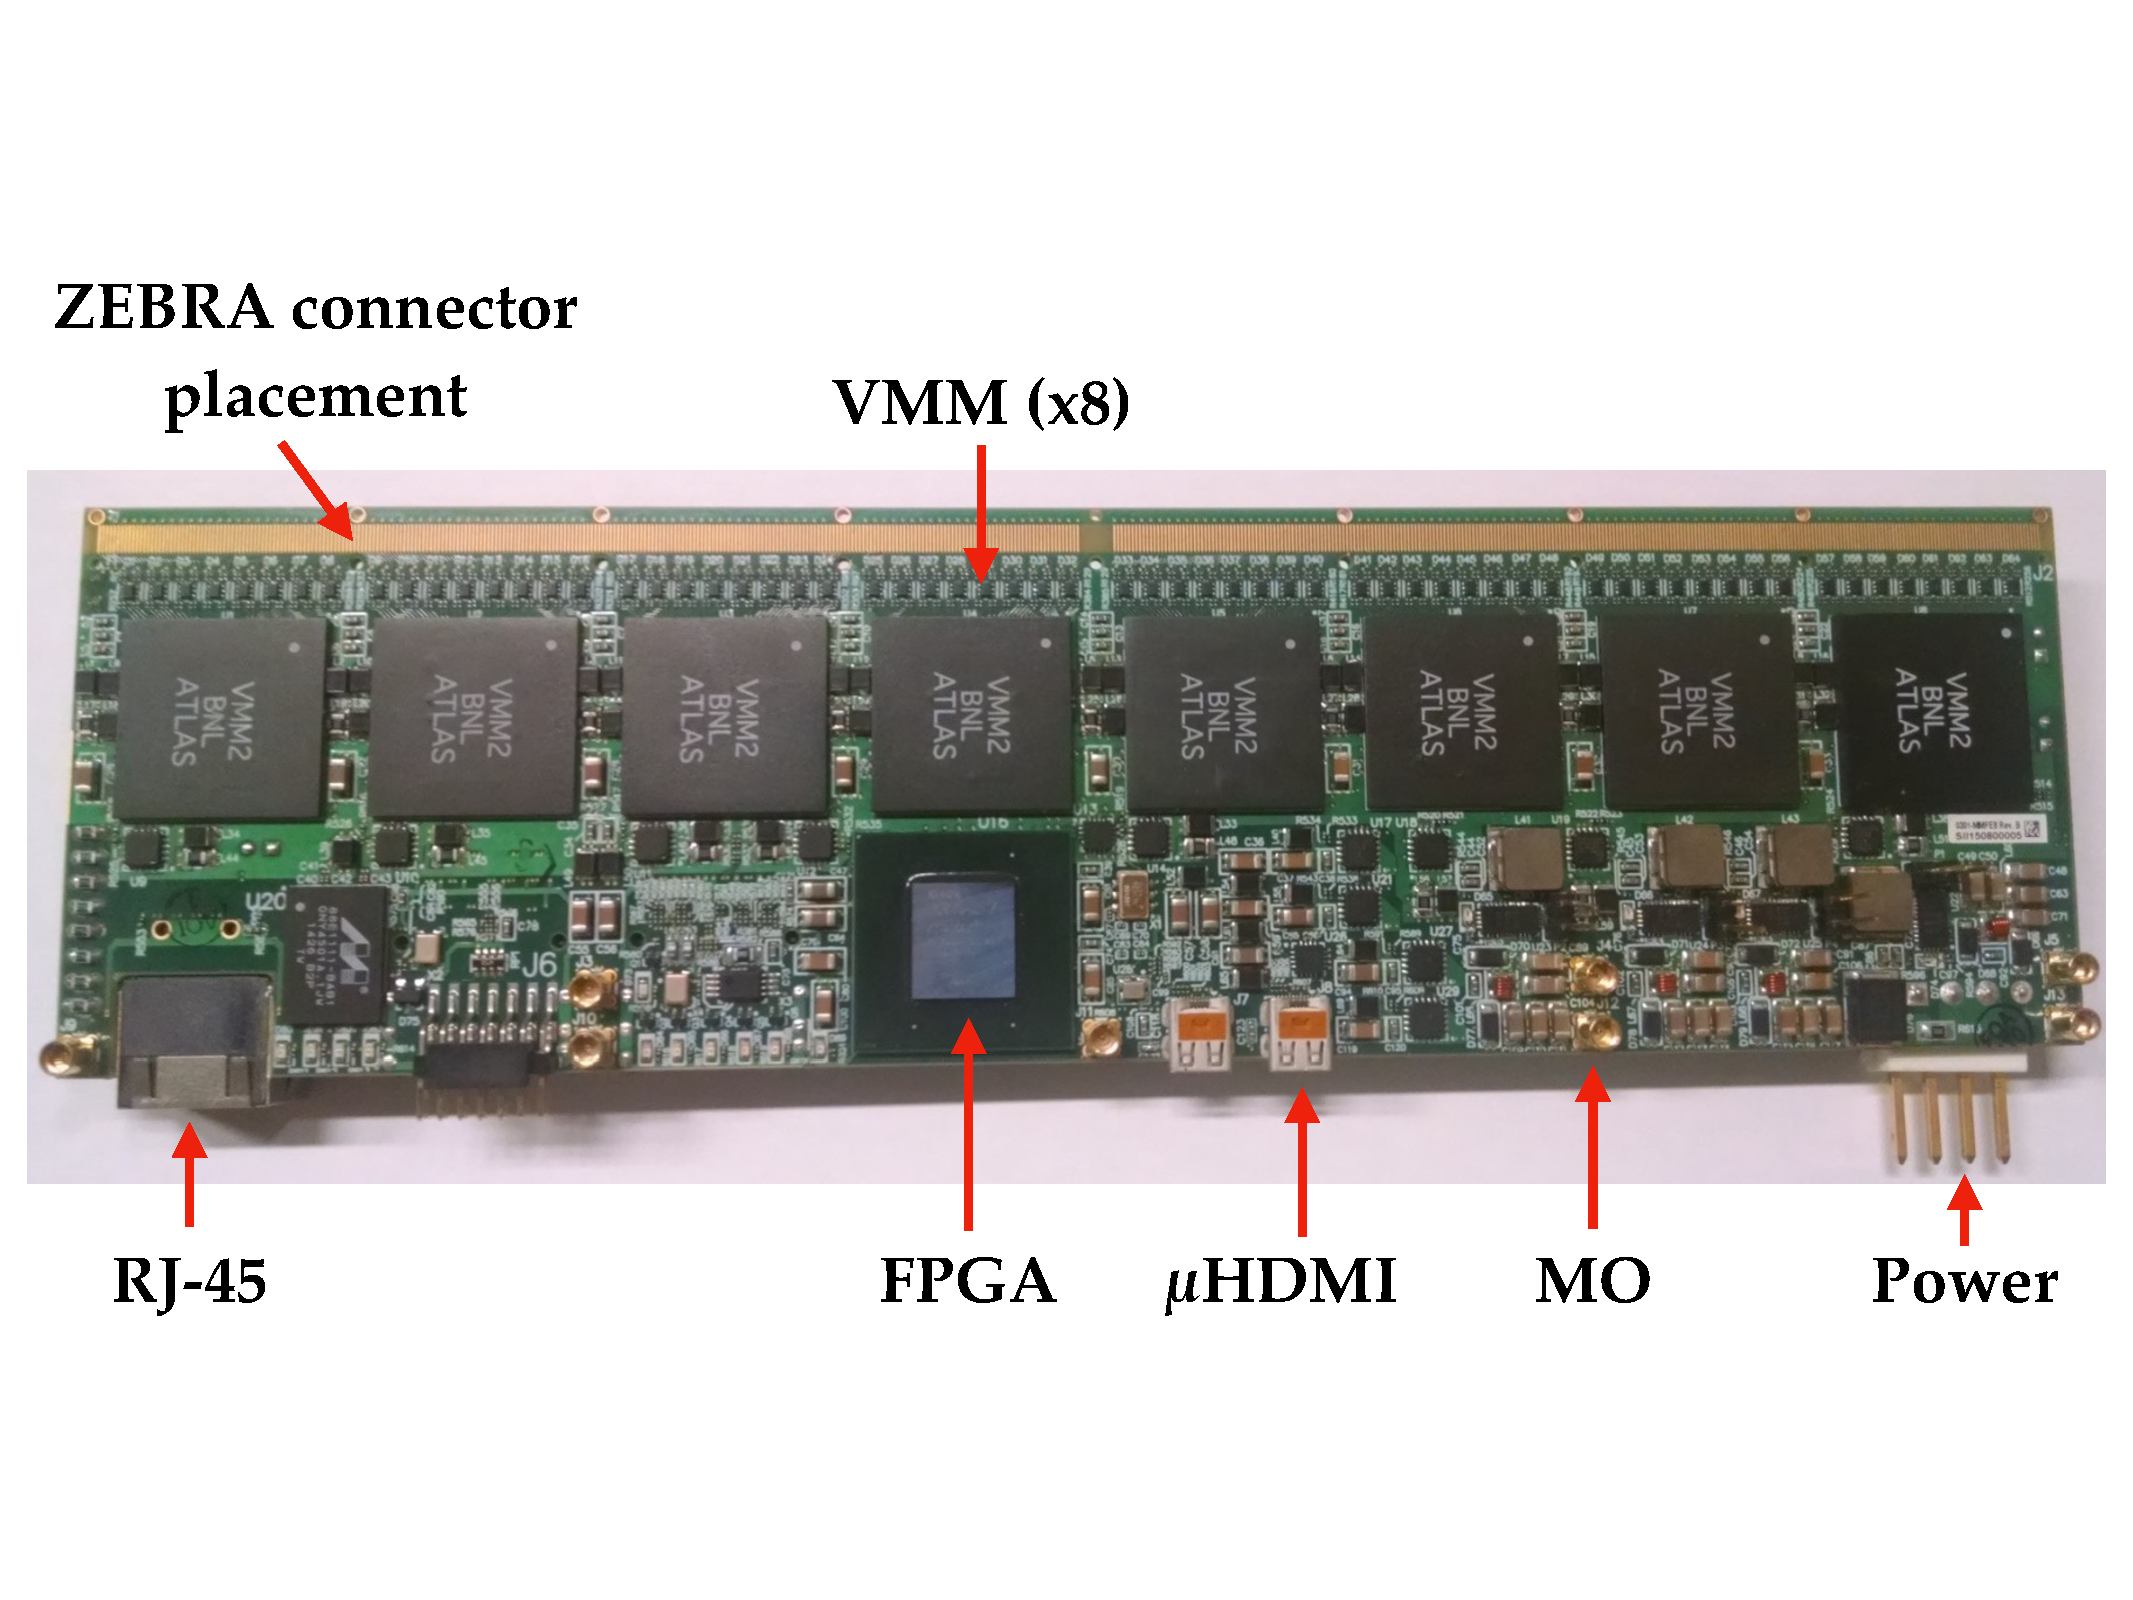
\includegraphics[width=0.8\textwidth]{figures/nsw/frontend/mmfe8_labelledPDF}
        \caption{
            Pictures of two VMM-based frontend boards. The RJ-45 connectors provide network I/O via
            standard Ethernet cables.
            The $\mu$HDMI connectors provide inputs for additional signalling purposes, such as external
            trigger signals.
            `MO' refers to the multiplexed monitoring output of the VMM (see Figure~\ref{fig:vmm3_channel}), which samples the analog
            signals internal to the VMM, such as the shaped input signals, prior to their digitisation.
            \textbf{\textit{Top}}: General purpose VMM (GPVMM) board housing a single VMM ASIC.
            The MO and trigger I/O are provided by LEMO connectors.
            \textbf{\textit{Bottom}}: Prototype MMFE8 board with its 8 VMM ASICs.
            The ZEBRA connector used for the MM detectors is described in the text.
            On this board the MO output is accessible primarily by the use of an oscilloscope probe.
        }
        \label{fig:frontend_boards}
    \end{center}
\end{figure}

\begin{figure}[!htb]
    \begin{center}
        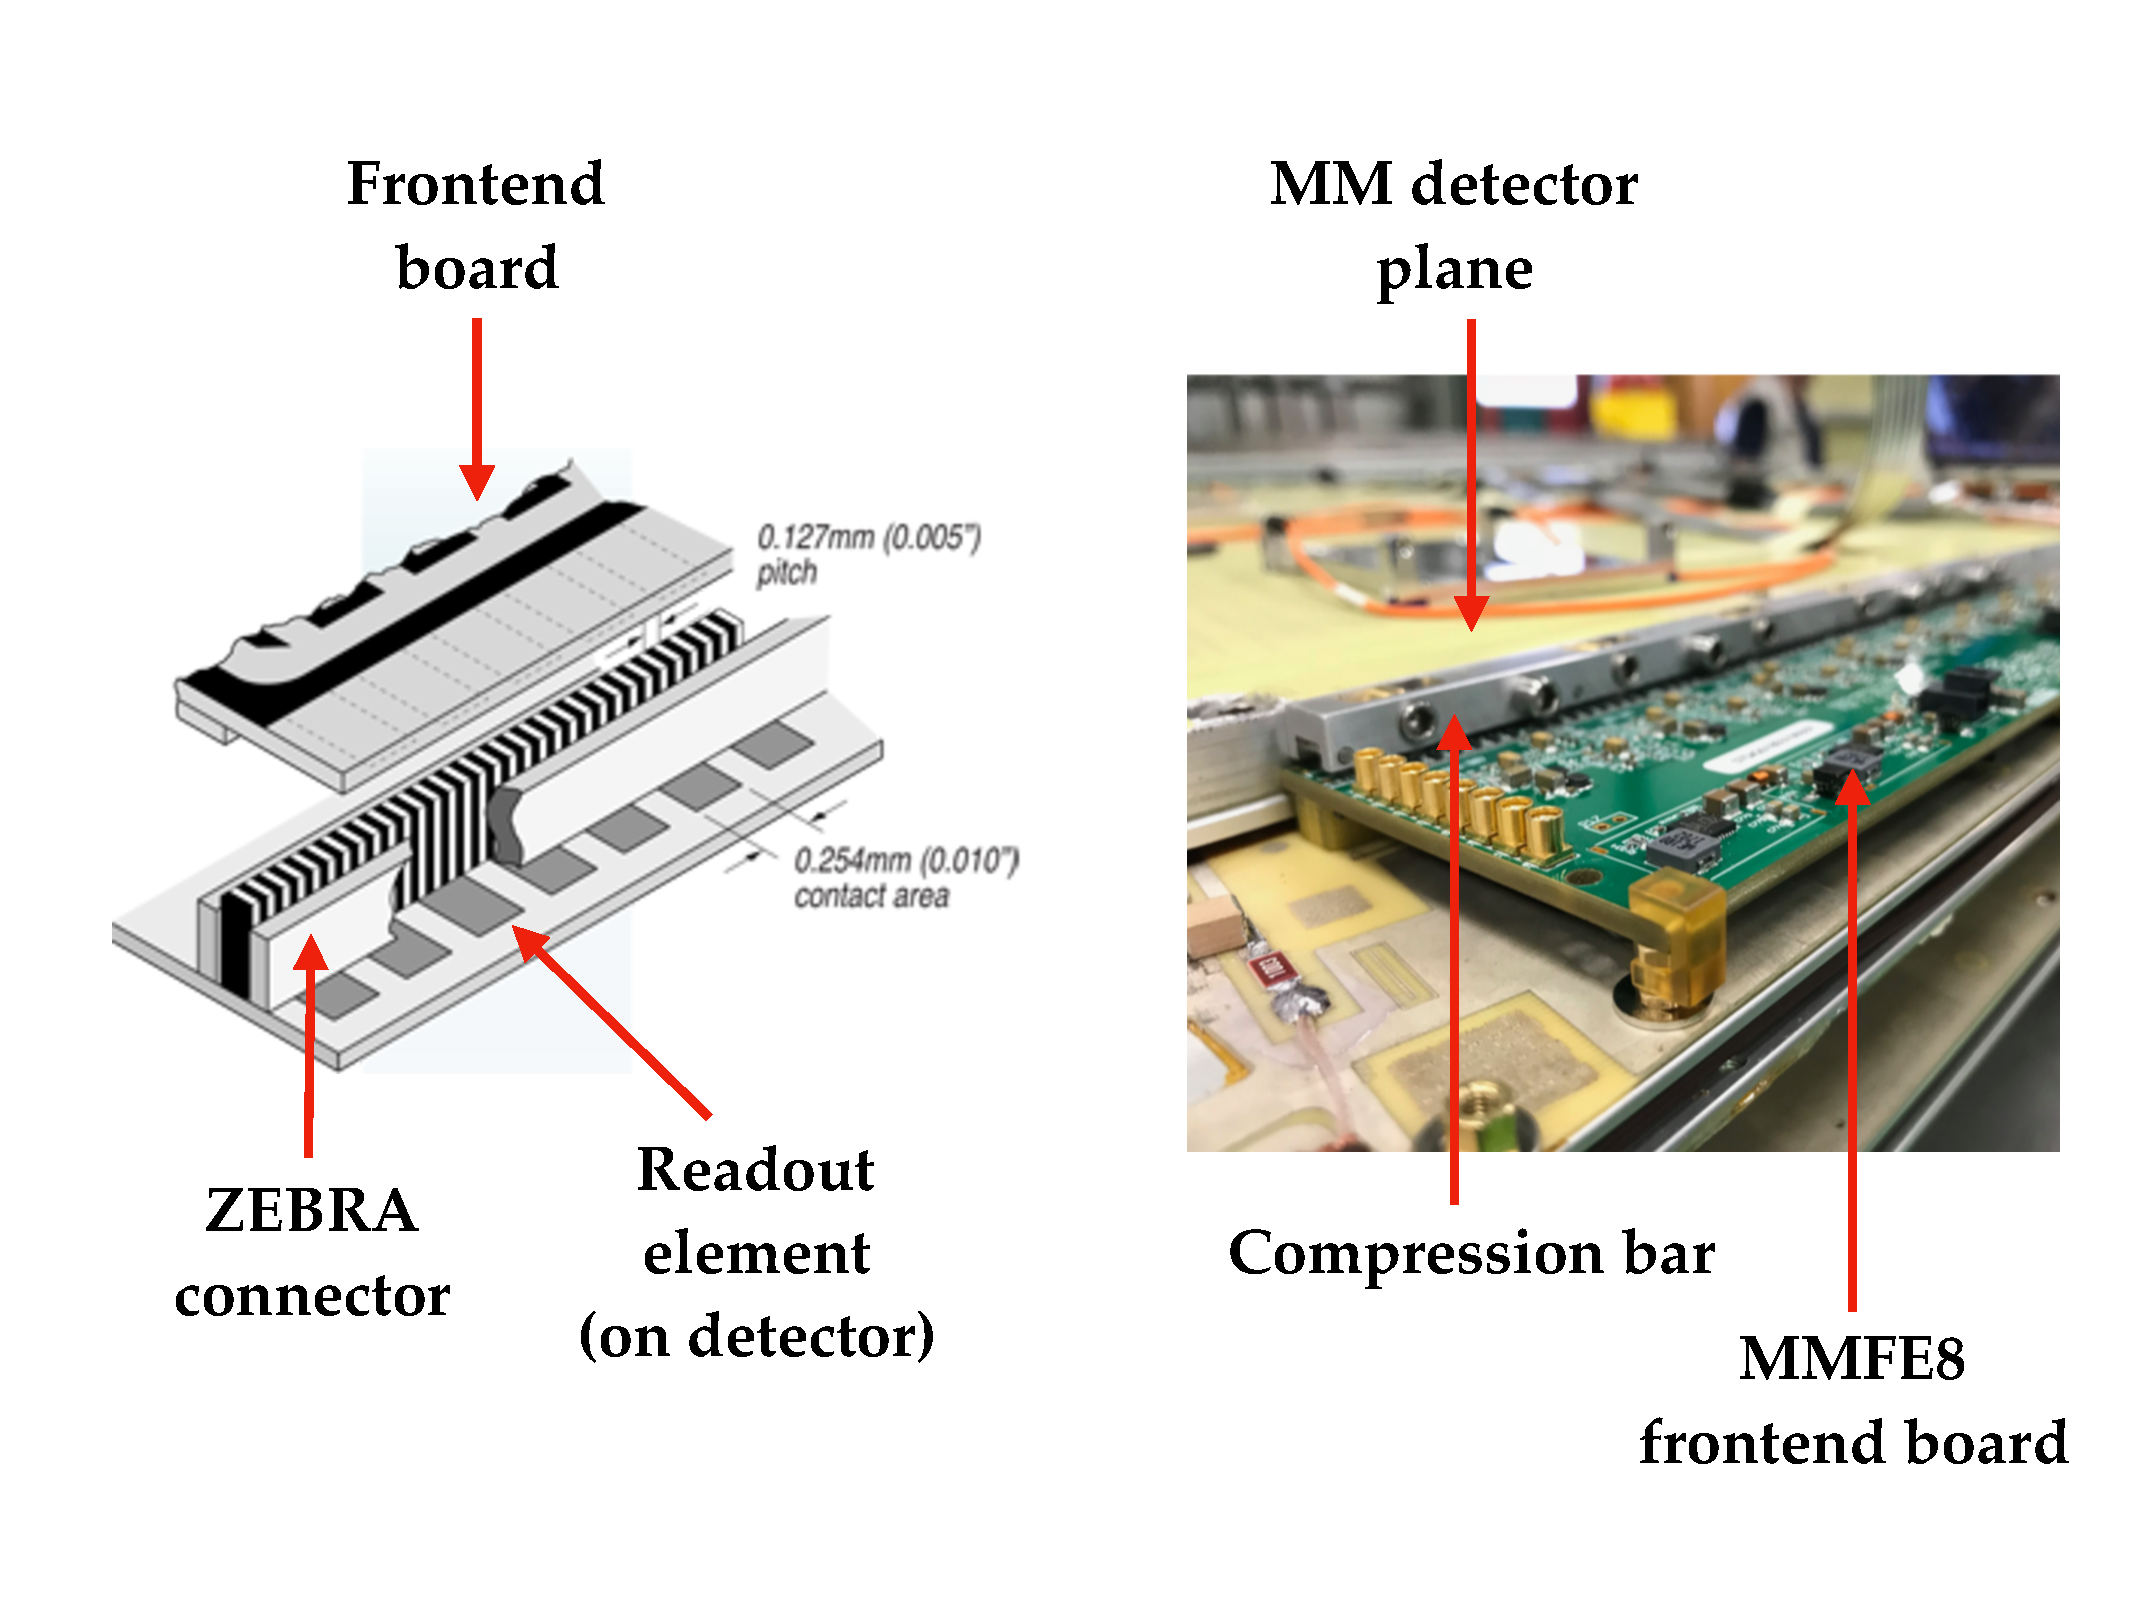
\includegraphics[width=0.8\textwidth]{figures/nsw/frontend/zebra_connector_illustratedPDF}
        \caption{
            \textbf{\textit{Left}}: Illustration of the ZEBRA connector concept.
                The ZEBRA connector is composed of a high density of alternating conductive (white) and non-conductive (black) layers
                that make contact with the detector readout elements on bottom and frontend board sensing elements
                on top.
            \textbf{\textit{Right}}: Picture of the ZEBRA connector being used with an MMFE8 frontend board
                on a full-scale MM detector.
                When interfaced to the MM detector, the MMFE8 frontend board is situated such that the VMMs are downward facing and
                are not therefore visible as pictured.
                The connection of the ZEBRA connector is realised via the tightening of a compression bar mounted on the MM detector chamber.
                The resulting
                downward pressure forces the ZEBRA connector to be securely sandwiched between
                the readout elements of the MM detector and VMM channel inputs located on the frontend board, bringing them in direct electrical contact.
        }
        \label{fig:zebra_connector}
    \end{center}
\end{figure}

The NSW frontend boards are interfaced directly to the detectors.
Both the GPVMM-type and MMFE8 frontend boards have been used on small prototype MM detectors, with
active area of $10\times10$\,cm$^2$.
A picture of an MMFE8 connected to such a detector is shown in Figure~\ref{fig:mmfe8_t2}.
On the full-scale MM detectors to be used in the NSW, the frontend boards are situated along the edge
of each detector layer in a given multilayer.
A drawing of a complete MM quadruplet with frontend electronics boards is shown in Figure~\ref{fig:mm_quad_elx}.


\begin{figure}[!htb]
    \begin{center}
        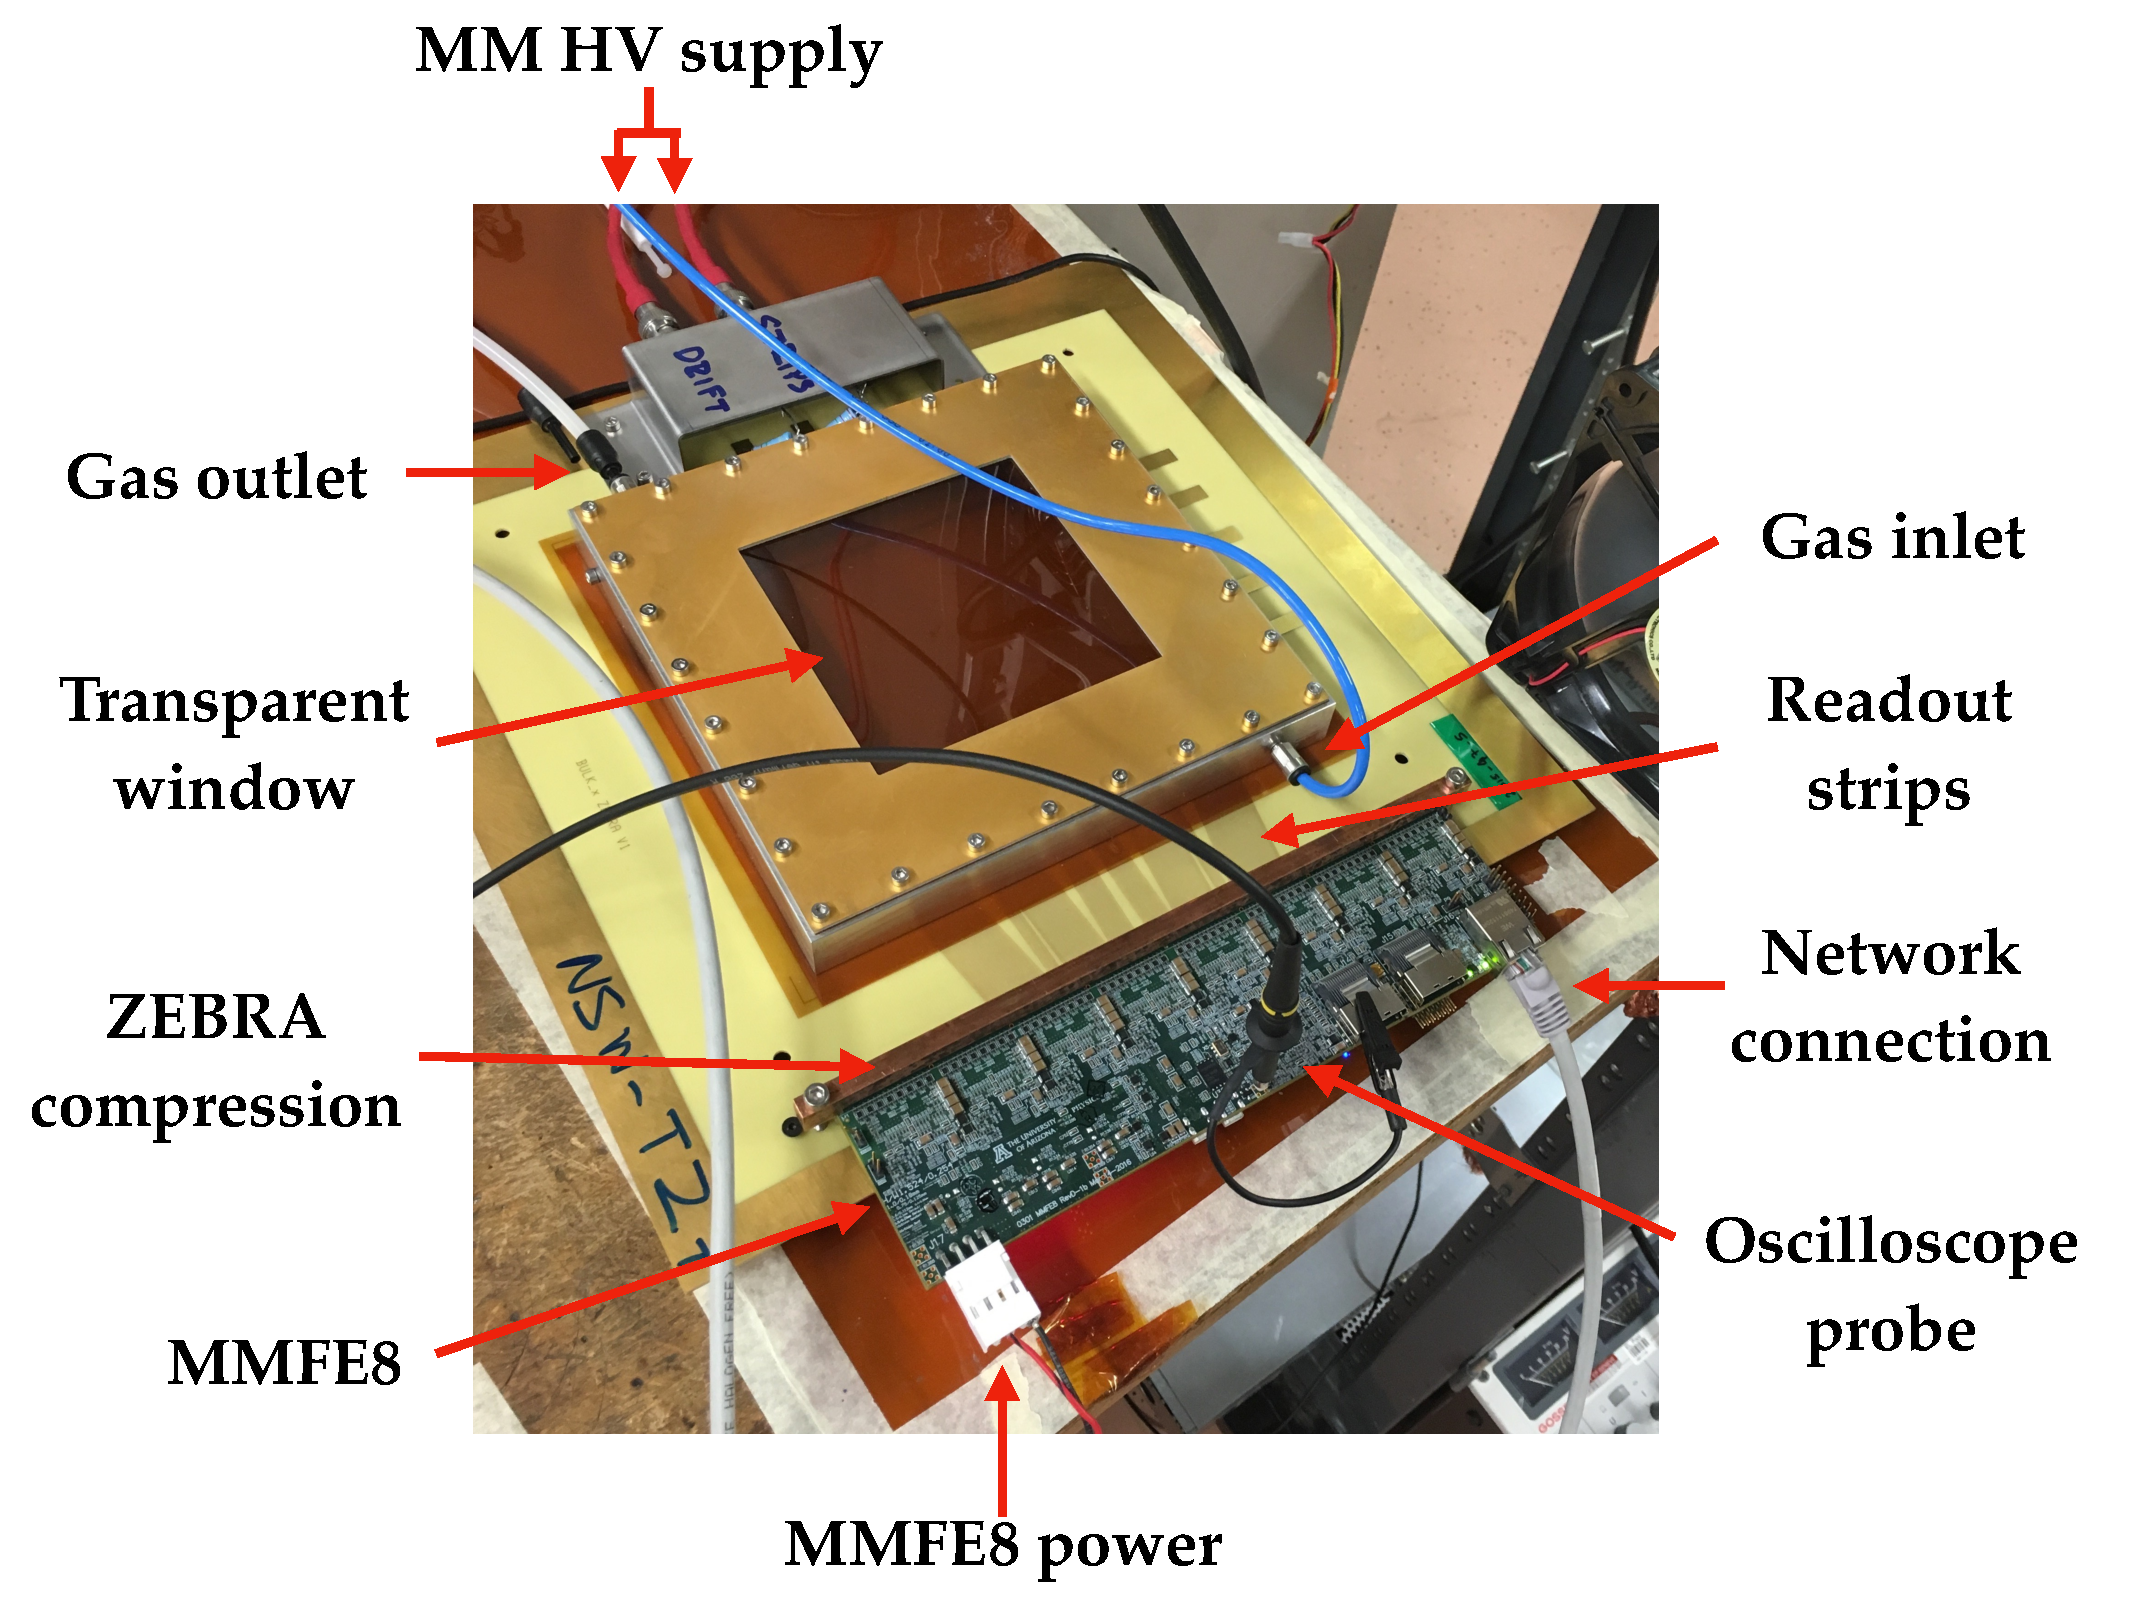
\includegraphics[width=0.7\textwidth]{figures/nsw/frontend/mmfe8_t2_labelledPDF}
        \caption{
            An MMFE8 interfaced to a small $10\times10$\,cm$^2$ prototype MM detector chamber
            in the RD51 lab at CERN.
            The transparent window allows for visual inspection of the drift mesh and
            reduction in material through which incident particles pass.
            The red cables at the top provide the high voltage (HV) power supply to the
            MM drift mesh and the resistive strips.
            The routing of the detector strips to the MMFE8 can be seen on the chamber backplane.
        }
        \label{fig:mmfe8_t2}
    \end{center}
\end{figure}

\begin{figure}[!htb]
    \begin{center}
        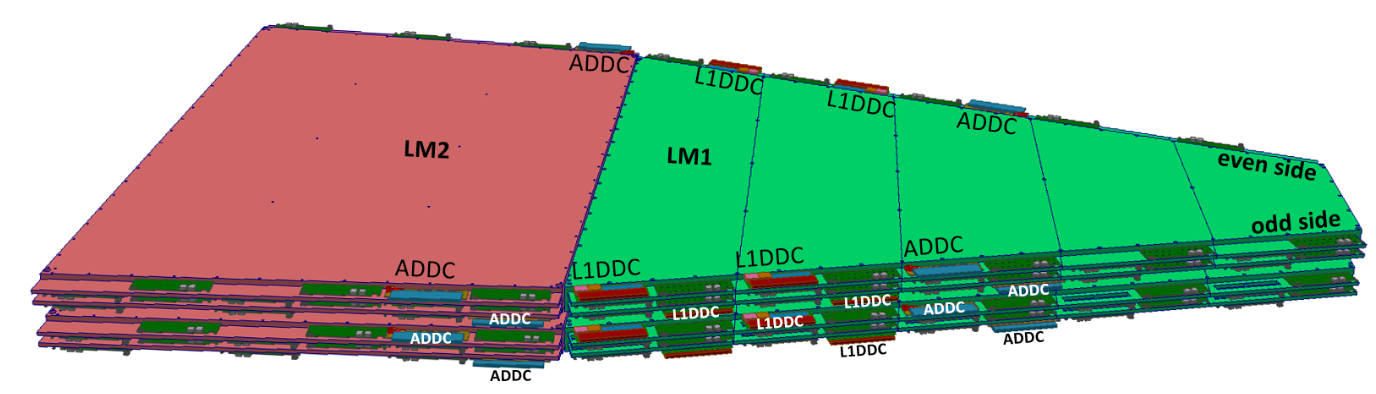
\includegraphics[width=0.6\textwidth]{figures/nsw/frontend/mm_quad_elx}
        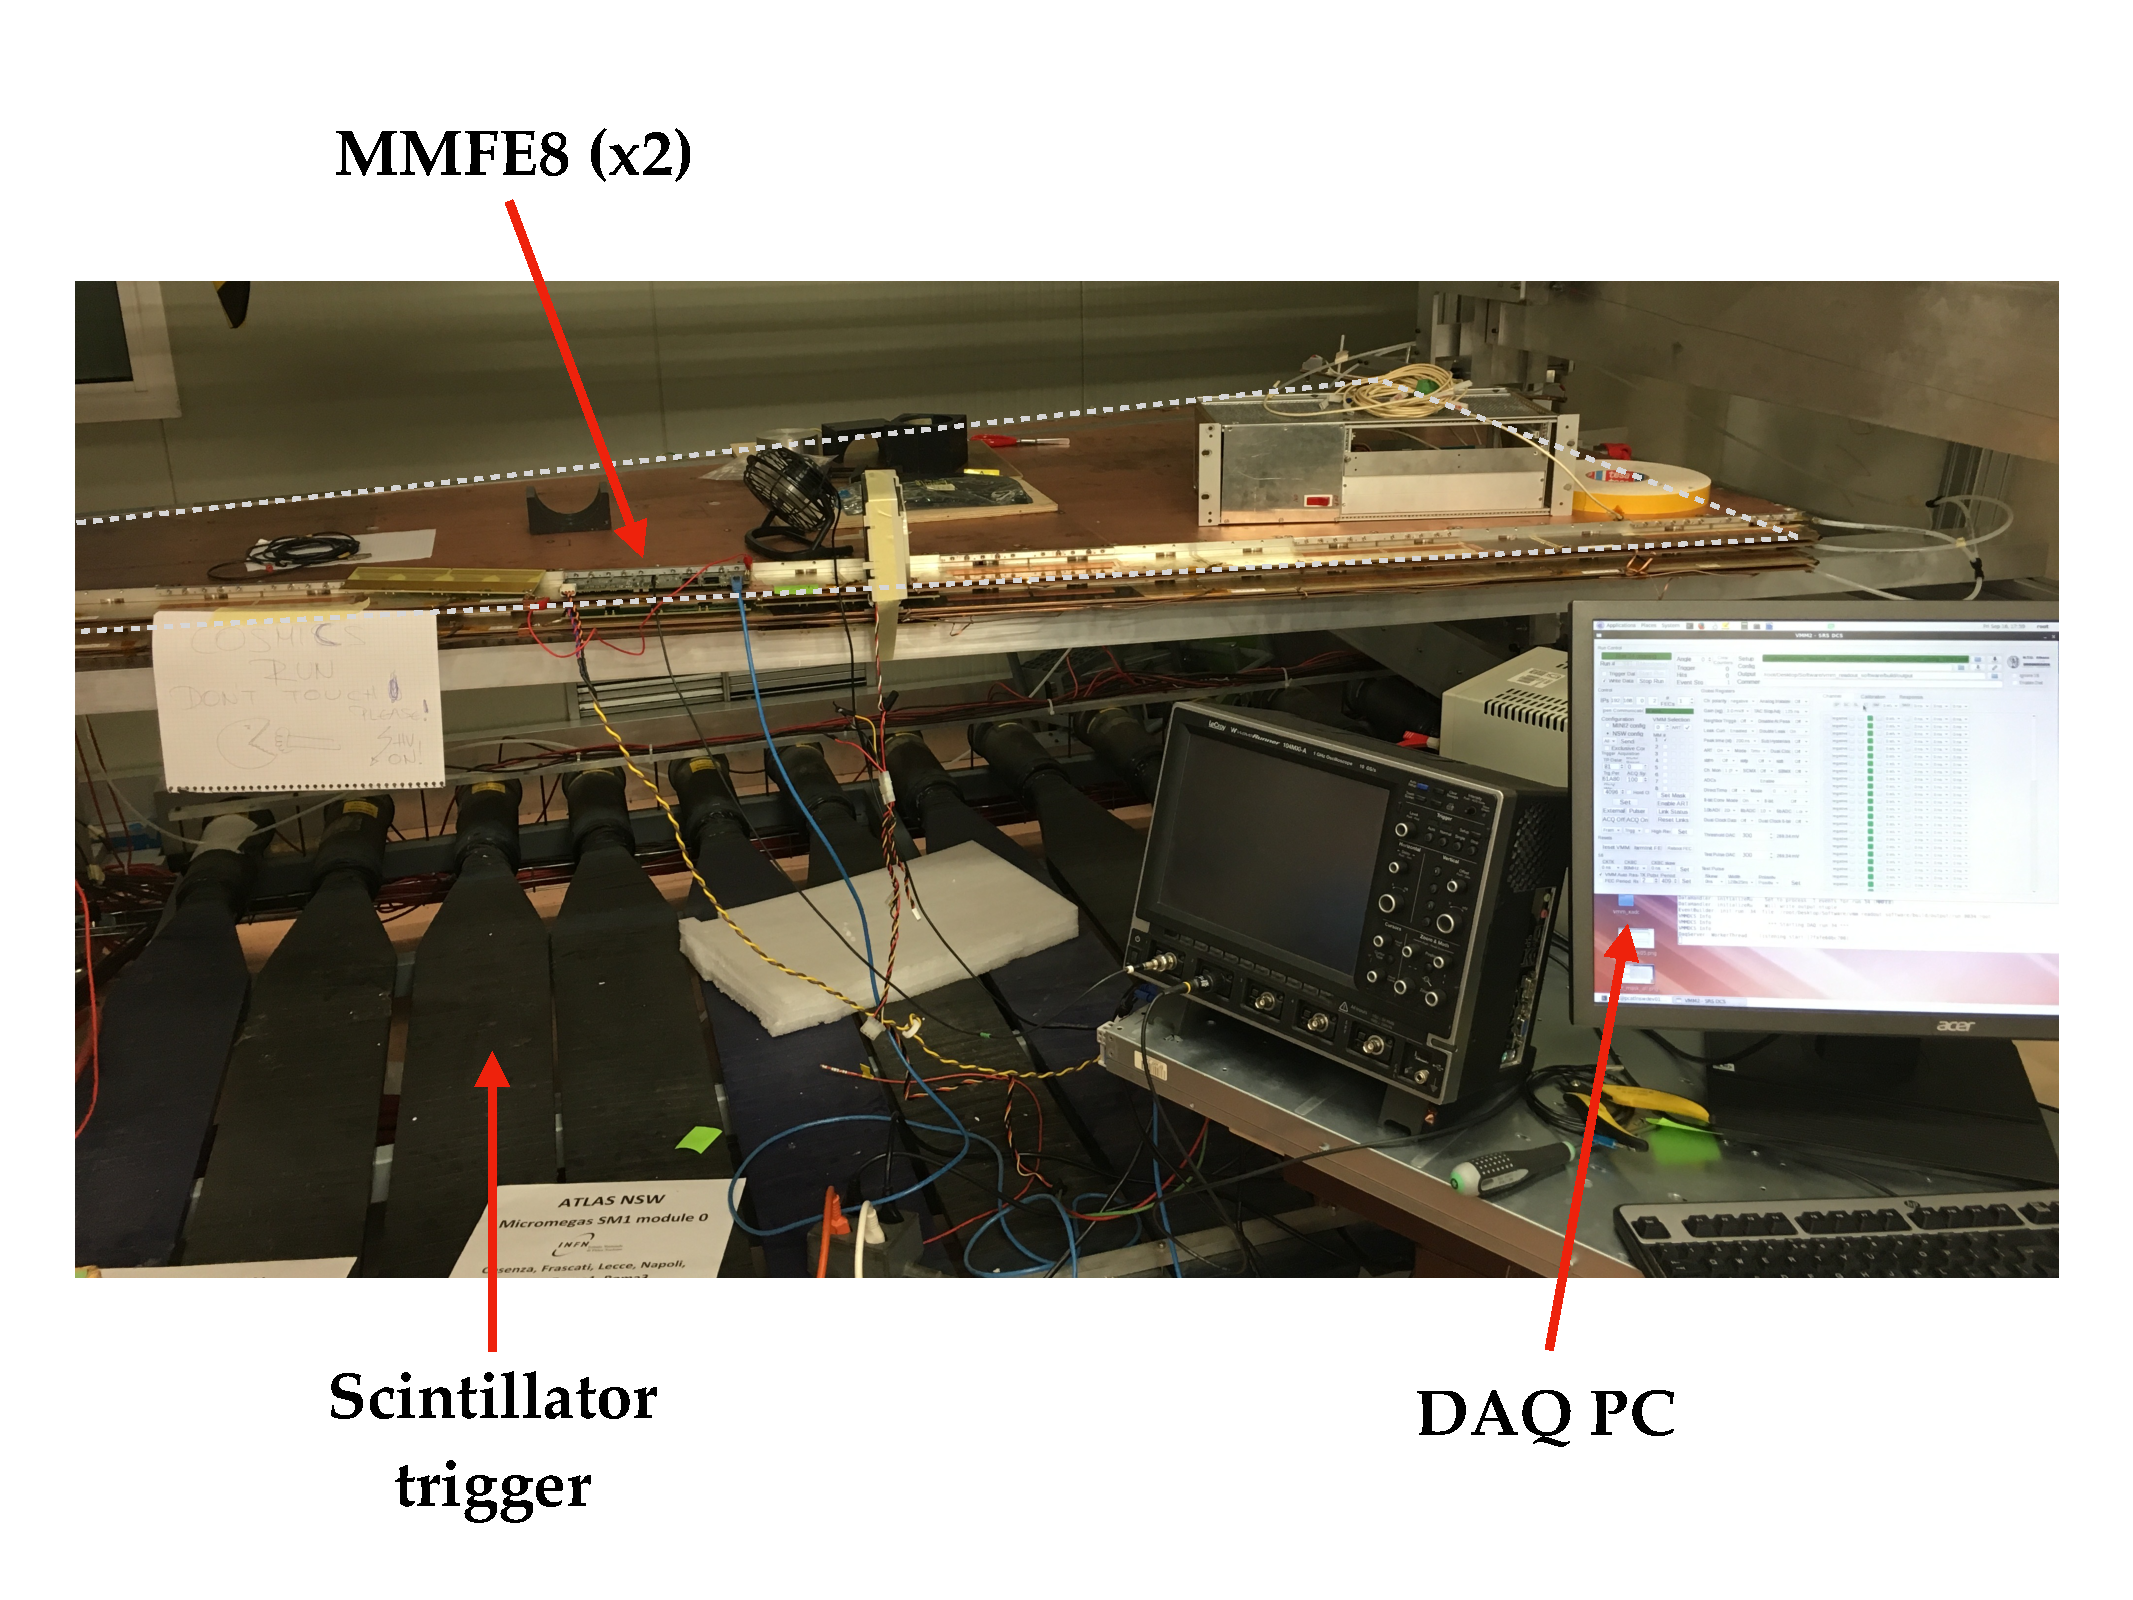
\includegraphics[width=0.48\textwidth]{figures/nsw/frontend/mmfe8_sm0_labelledPDF}
        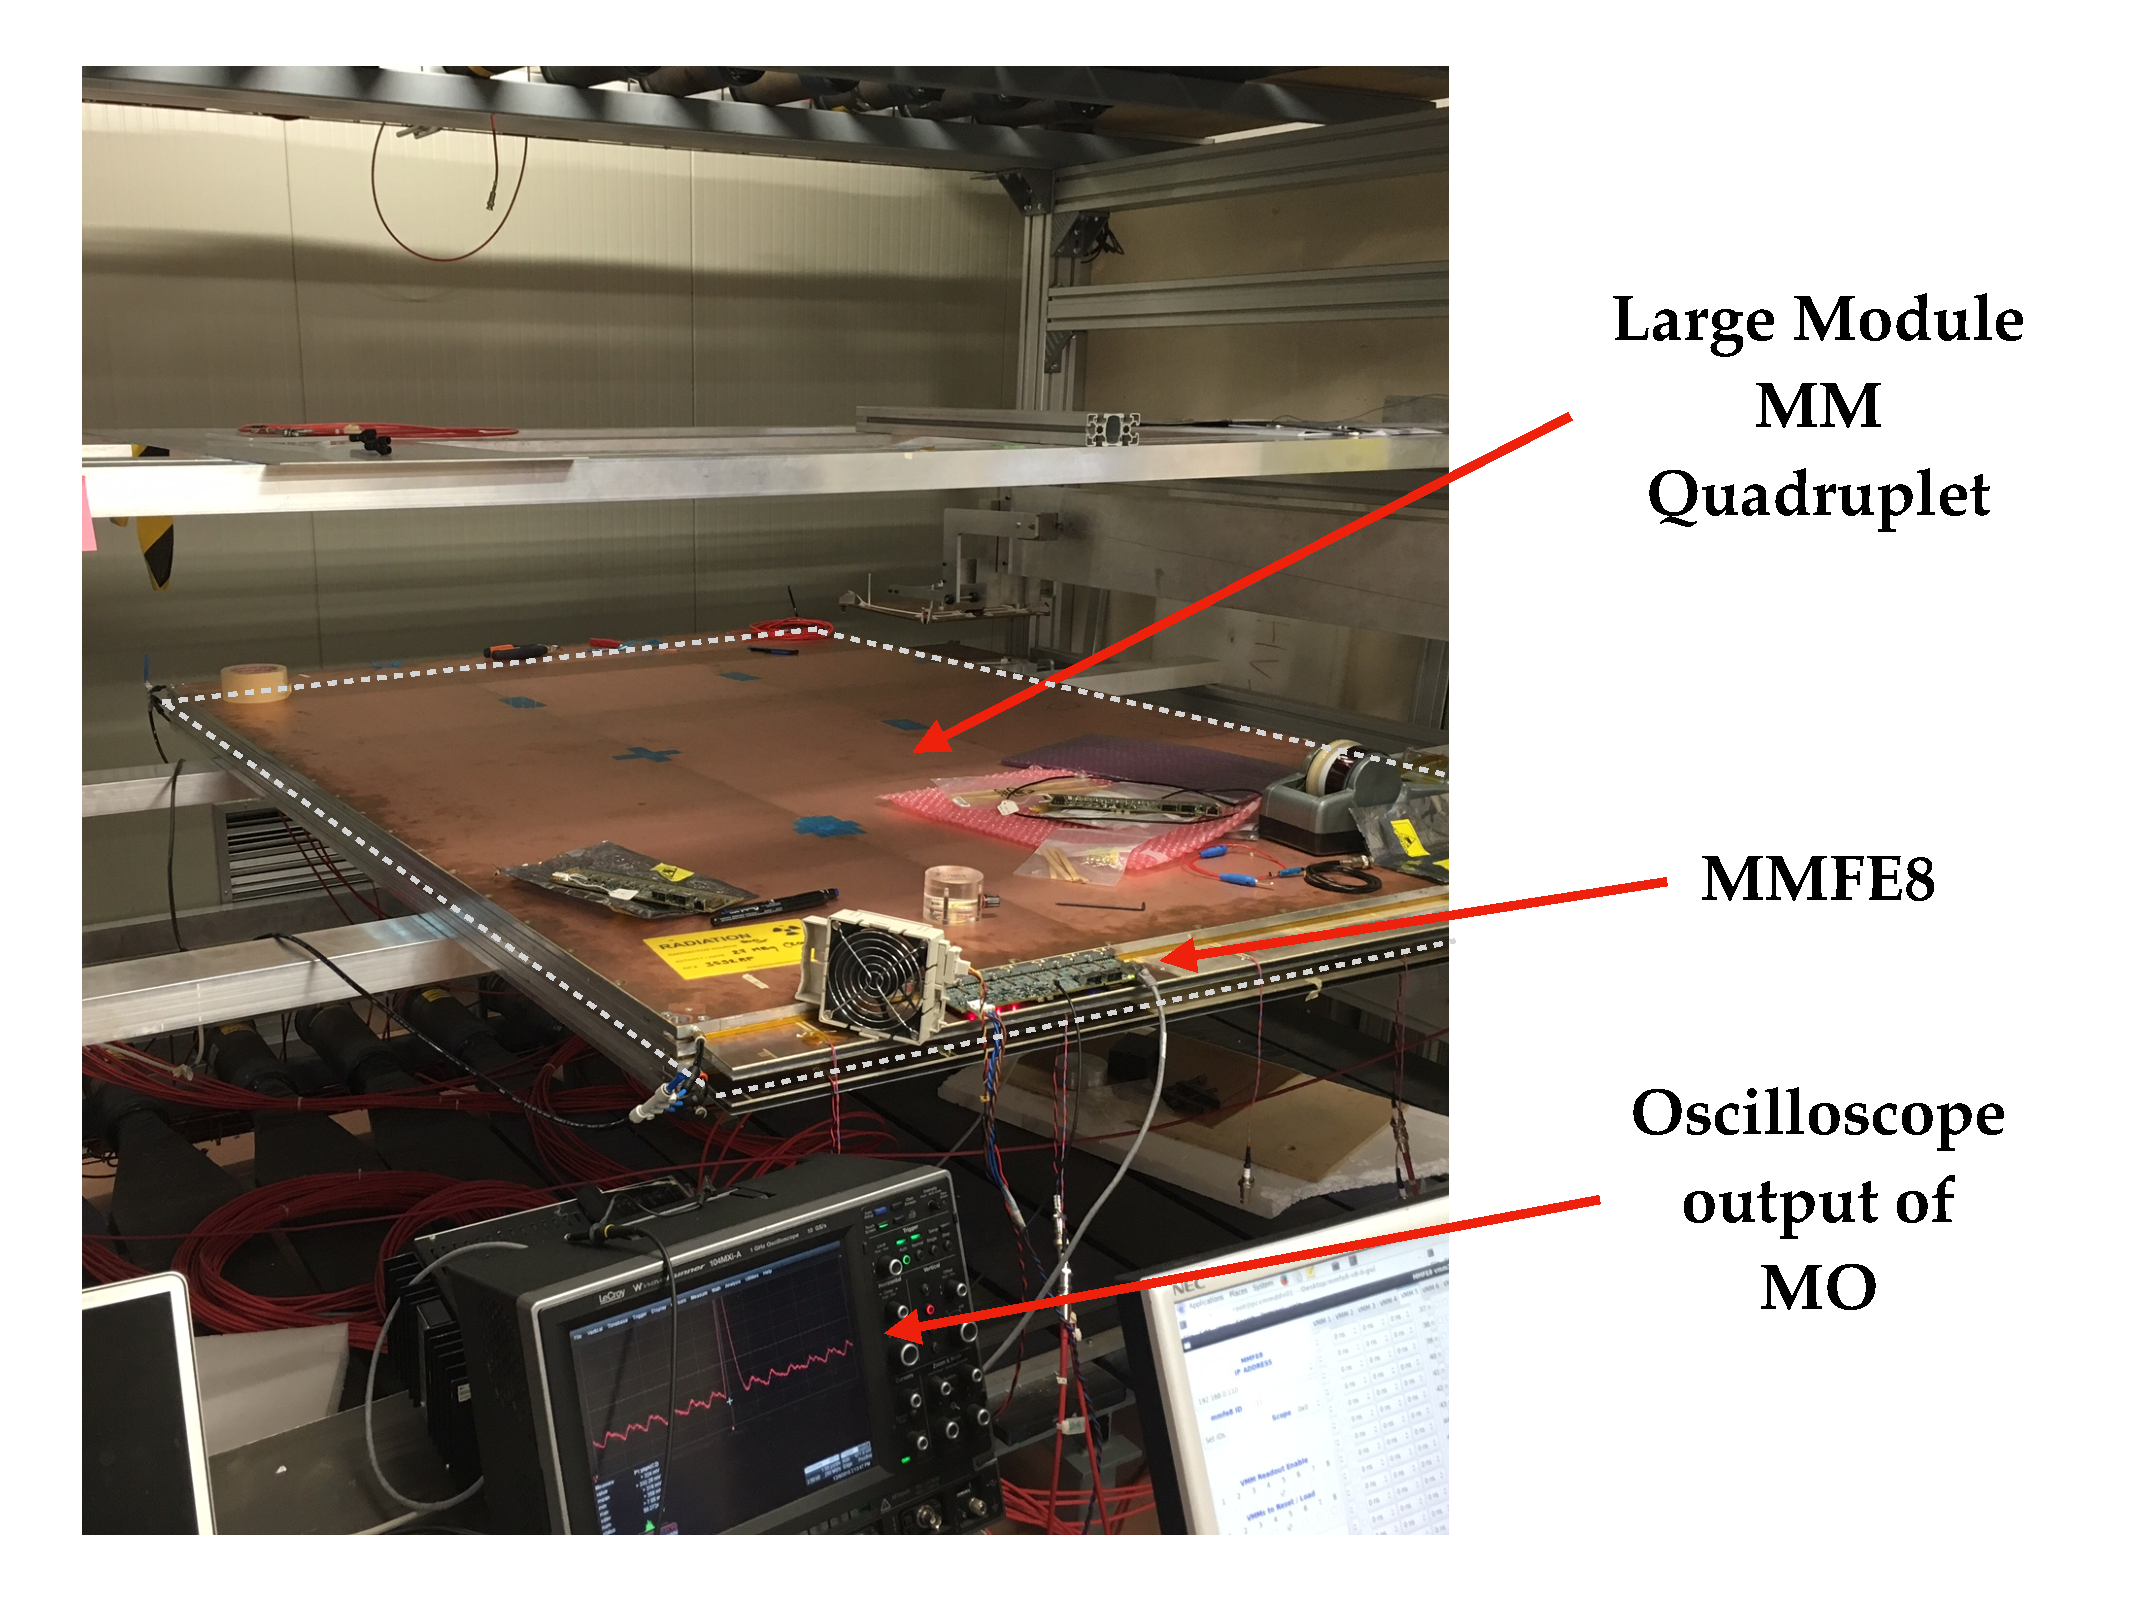
\includegraphics[width=0.48\textwidth]{figures/nsw/frontend/mmfe8_lm2_labelledPDF}
        \caption{
            \textbf{\textit{Top}}: Mechanical drawing of a MM large sector quadruplet.
                MM quadruplets are segmented into two modules, here indicated as LM1 and LM2.
                Indicated along the edge of the quadruplet are the locations of the frontend boards
                interfaced directly with the detector.
                The green frontend boards are the MMFE8s housing the VMM ASICs.
                Information about the L1DDC and ADDC boards can be found in Ref.~\cite{NSWFrontEndChristos}.
            \textbf{\textit{Bottom, left}}: The first small-sector MM quadruplet module (only the lower half, analogous to the LM1 in the Top drawing), `SM0', on the cosmic-ray
                test-stand located in the RD51 lab at CERN.
                The SM0 module is partially instrumented, with only a few MMFE8 boards interfaced
                as indicated.
                The outline of the SM0 module is given by the grey dashed line.
                The lower half of the scintillator-trigger system is seen beneath the SM0 module.
            \textbf{\textit{Bottom, right}}: The first LM2-type MM quadruplet module on the cosmic-ray
                test-stand located in the RD51 lab at CERN.
                The outline of the LM2 module is given by the grey dashed line.
                A shaped VMM signal pulse can be seen on the oscilloscope.
        }
        \label{fig:mm_quad_elx}
    \end{center}
\end{figure}
